\section{Problema clasificării. Tipuri de clasificare}
\subsection{Învățare supervizată}
În contextul învățării supervizate ne este pus la dispoziție un set de date format din perechi $(x_i, y_i)$, $x_i$ numindu-se \textit{instanță} și $y_i$ \textit{etichetă}. Obiectivul unui algoritm de învățare automată este de a învăța o funcție care să modeleze cât mai bine relația dintre $x_i$ și $y_i$ ce reiese din date. După natura variabilei $y$, se pot defini 2 tipuri de probleme:

\begin{itemize}
\item Clasificare (variabila $y$ este discretă)
\item Regresie (variabila $y$ este continuă)
\end{itemize}

În această lucrare vom aborda doar subiectul clasificării.

\subsection{Clasificare binară}
Problema clasificării binare ne cere ca pentru o instanța $x\in\mathbb{R}^p, \ p\in\mathbb{N^*}$  dată ca input și o clasă $C$, să returnăm o valoare $y\in\{0, 1\}$ astfel încât $y=1$ dacă $x$ face parte din clasa $C$, sau $y=0$ în caz contrar. Mai formal, trebuie să gasim o funcție $h:\mathbb{R}^p\rightarrow\{0, 1\}$ definită astfel: 

\[
h(x)=
	\begin{cases}
		\text{1,} &\quad\text{x}\in\text{C} \\
		\text{0,} &\quad\text{altfel.} \\
	\end{cases}
\]

Această funcție se mai numește model sau ipoteză și scopul unui algoritm de învățare automată este de a oferii un model cât mai bun.\\
Un exemplu de clasificare binară este ca pentru o imagine să decidem dacă în aceasta se află sau nu o pisică. În acest caz, instanța $x$ va fi un vector ce conține valoarea reală a fiecarui pixel și output-ul va fi $y=1$ dacă în imagine apare o pisică sau $y=0$ în caz contrar.

\subsection{Clasificare cu clase multiple}
La fel ca în cazul clasificării binare, instanța este $x\in\mathbb{R}^p, \ p\in\mathbb{N^*}$, însă, în loc de o singură clasă $C$, avem o mulțime $\{C_1,C_2,...,C_k\} \; k\in\mathbb{N^*}$ disjuncte, iar obiectivul este să găsim o funcție $h:\mathbb{R}^p\rightarrow\{0,1,2,...,k\}$ astfel încât:

\[
h(x)=
	\begin{cases}
		\text{1,} &\quad\text{x}\in\text{$C_1$} \\
		\text{2,} &\quad\text{x}\in\text{$C_2$} \\
		\vdots &\quad\quad\vdots \\
		\text{k,} &\quad\text{x}\in\text{$C_k$} \\
		\text{0,} &\quad\text{altfel.} \\
	\end{cases}
\]

\subsection{Clasificare cu etichete multiple}
Pentru o instanță definită la fel ca mai sus $x\in\mathbb{R}^p, \ p\in\mathbb{N^*}$ și o mulțime $C=\{C_1,C_2,...,C_k\} \; k\in\mathbb{N^*}$ vom construi o ipoteză $h:\mathbb{R}^p\rightarrow\{0, 1\}^k$ astfel încât pentru o predicție $y=h(x)$ să avem:

\[
y_i=
	\begin{cases}
		\text{1,} &\quad\text{x}\in\text{$C_i$} \\
		\text{0,} &\quad\text{altfel.} \\
	\end{cases}
\quad i=\overline{1,k}
\]

Apare des o confuzie între clasificarea cu etichete multiple și cea cu clase multiple. Diferența fundamentală este că în prima o instanță poate să aparțină mai multor clase, spre deosebire de cealaltă, în care o instanță este asignată unei singure clase. Totodată, clasificarea binară este un caz particular a clasificării cu etichete multiple atunci când $k=1$. Detectarea obiectelor face parte din acest tip de clasificare, unde, pentru o imagine, vom marca prezența mai multor obiecte (clase) și nu a unui singur element.

\subsection{Învățare multi-instanță}
În acest caz, o instanță nu mai este reprezentată de un singur vector de numere reale, ci de o mulțime de astfel de vectori. Fie $X=\{x_1, x_2,...,x_k\}, \ k\in\mathbb{N^*}, \ x_i\in\mathbb{R}^{p_i}, \ p_i\in\mathbb{N^*}$ o instanță. O ipoteză $h$ determinată de un algoritm de învățare automată va clasifica întreaga mulțime $X$ și nu fiecare componentă $x_i$ independent \cite{multiInstance}.   \\

Problema abordată în această lucrare este una de învățare multi-instanță și de clasificare cu etichete multiple. Un restaurant este reprezentat de o mulțime de imagini și rezultatul este un vector $y$ cu 9 componente, fiecare marcând prezență sau absență celor 9 clase descrise în capitolul introductiv.\\


\begin{tabular}{lll}
\raisebox{-.5\height}{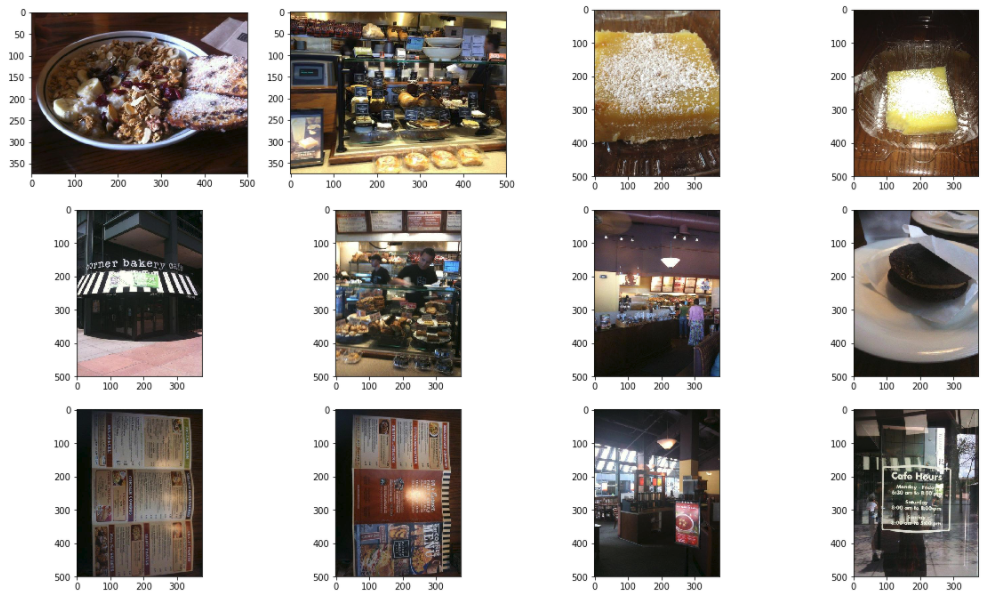
\includegraphics[scale=0.3]{restaurantInstance.png}} & 
\begin{Huge}
	$\rightarrow$
\end{Huge} &
\begin{Large}
	$y=[1, 0, 0, 1, 1, 0, 1, 1, 0]$
\end{Large}\\
\end{tabular}

\begin{center}
Figura 1: O instanță formată din 12 fotografii și vectorul asociat
\end{center}